\subsubsection{Архитектура Системы}

Учитывая опыт существующих разработок, направленных на решение поставленной задачи, а особенности {\it VBA} и {\it VSTA}, Была разработана концептуальная модель взаимодействия основных компонентов платформы.

\subsubsection{Пару слов о выбранных технологиях}

В качестве внешней IDE для разработки расширений была выбрана IDE с открытым исходным кодом SharpDevelop. Этот выбор был сделан по нескольким причинам:

Во-первых, эта IDE может управляться программно извне при помощи встроенной технологии SDA. Программное управление позволяет выполнять различные действия в IDE без участия пользователя. Например, показывать или скрывать само приложение, запускать сборку проекта, управлять сохранением и загрузкой проектов, и многие другие. 

Во-вторых, эта IDE поддерживает плагины. Это свойство позволит добавить какую-либо отсутствующую в базовой поставке функциональность не меняя исходного кода самого SharpDevelop. Это важно, так как изменение исходного кода сделает неудобным распространение готовой платформы, так как она будет совместима только с конкретной сборкой SharpDevelop. Использование плагинов позволит добавить нужную функцинальность в уже установленный экземпляр этой IDE.

В-третьих, SharpDevelop поддерживает кастомизацию, то есть изменение своего внешного вида и поведения при момощи конфигурационных файлов. Под изменением внешнего вида нужно понимать удаление <<лишних>> в контексте данного сценария использования (как внешней IDE для разработки расширений) элементов управления, добавление новых элементов управления, управление доступностью этих элементов, и прочее. Изменение поведения состоит в подмене штатных обработчиков событий элементов управления (например, кнопок), на свои собственные обработчики с измененной логикой. Например, запуск отладчика не должен пытаться стартовать сборку самого расширения (это попросту невозможно, так как расширения представляет из себя библиотеку классов), а присоединить отладчик к процессу хост-приложения.

В-четвертых, открытый исходных код поможет быстрее решить проблемы, связанные с интеграцией SharpDevelop в разрабатываемую платформу, так как сама IDE может быть запущена под отладчиком.

Как видно на рисунке \ref{fw_arch1}, система состоит из двух отдельных процессов. Такая архитектура обусловлена необходимостью поддержку отладки расширений, а отладчик, как известно, должен выполняться в отдельном процессе. Кроме того, хост-процесс IDE является дочерним для процесса хост-приложения. Управление этими процессами организовано таким образом, что в случае прекращения из-за критической ошибки работы процесса, обслуживающего IDE, этот процесс будет автоматически перезапущен. В таком случае систама продолжит работу в штатном режиме. Напротив, при сбое в процессе хост-приложения, будет остановлен так же хост-процесс IDE, что позволяет предотвратить возникновения в системе <<паразитных>> процессов.

\begin{figure}[!h]
    \centering
    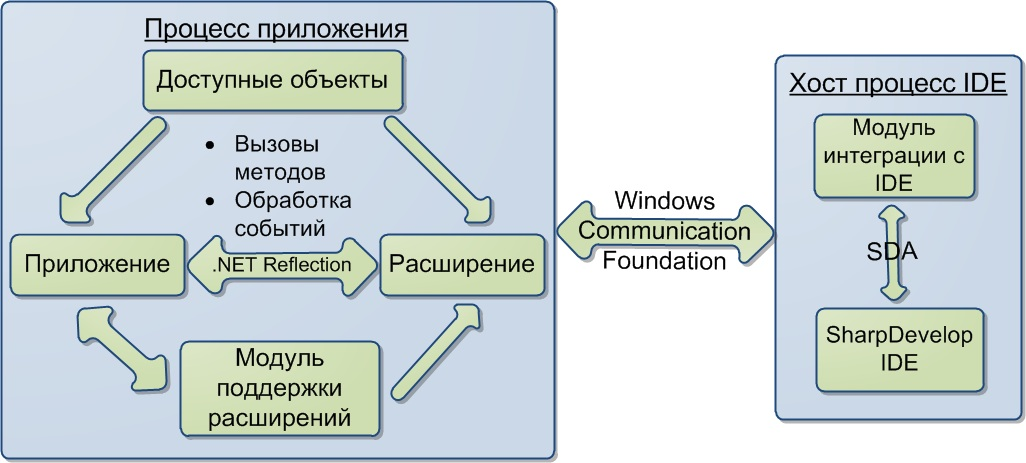
\includegraphics[width=15cm]{fw_arch1.jpg}
    \caption{Взаимодействие компонентов системы}
    \label{fw_arch1}
\end{figure}

Меж-процессное взаимодействие в разрабатываемой системе было решено реализовать при помощи именнованных каналов {\tt (named pipe)} из библиотеки WCF (Windows Communication Foundation). Выбор WCF обусловлен тем, что эта библиотека входит в состав .NET Framework, и использование ее будет наиболее оправдано для разработки приложения под эту платформу. Реализация именнованых каналов в WCF --- NetNamedPipe, выбрана по причине того, что в рамках решения задачи по обеспечению взаимодействия двух процессов на локальной машине нет необходимости в использовании более сложных и емких механизмов взаимодейчтвия, чем именнованые каналы.

Взаимодействие между процессами происходит по двум отдельным именнованым каналам, так как инициировать запросы (то есть выступать в роли сервера) могут оба процесса, и механизм <<запрос --- ответ>> в данном случае не подходит.

Более того, адреса, по которым взаимодействуют процессы выбираются случайно, что позволяет без возникновения конфликтов запускать множество пар процессов <<приложение --- IDE>>. Такое решение позволит использовать разрабатываемую платформу в нескольких приложениях одновременно.

\TODO{Может, нужно еще добавить про то, как обыно делают cross-thread communication?}

\subsubsection{Это у нас было сделано хоть как-то}

\TODO{Глава про взаимодействие с расширением(пока рефлекшн)}

\TODO{Глава про тулы для хост-приложения (гуй всякий)}

\TODO{Схема с более подробной архитектурой}

\TODO{ISO storage не забыть}

\TODO{Глава про кастомизацию \#D}

\TODO{Глава про допиливание \#D (например, бряки + сигнатуры)}

\TODO{Про реализацию всей этой байды, диаграммы классов, итд}

\subsubsection{Это пока вообще не сделано}

\TODO{Интеграция. Тут у нас ничего нет пока.}

\TODO{Зависимости расширений (это вроде модно сейчас)}

\TODO{Сравнение с аналогами}

\TODO{Бла-бла, как все хорошо получилось}
